%!TEX root = ../Thesis.tex

% 1.1 Background
% The background sets the general tone for your thesis. It should make a good impression and convince the reader why the theme is important and your approach relevant. Even so, it should be no longer than necessary.

% What is considered a relevant background depends on your field and its traditions. Background information might be historical in nature, or it might refer to previous research or practical considerations. You can also focus on a specific text, thinker or problem.

% Academic writing often means having a discussion with yourself (or some imagined opponent). To open your discussion, there are several options available. You may, for example:

% refers to a contemporary event
% outline a specific problem; a case study or an example
% review the relevant research/literature to demonstrate the need for this particular type of research
% If it is common in your discipline to reflect upon your experiences as a practitioner, this is the place to present them. In the remainder of your thesis, this kind of information should be avoided, particularly if it has not been collected systematically.

% Tip: Do not spend too much time on your background and opening remarks before you have gotten started with the main text.





\section{Background}
Coming from the field of telecommunication, through microwave engineering and electrical systems in satellites in last years I have focused on electric cars. After taking classes on electric vehicles I had my first practical experience by correcting the wire harness of converted to an electric off-road car. Afterwards, I worked on the electric conversion of the car towards the racing application.

\noindent
Both systems, although interesting, took an approach to use already designed solutions and did not require additional control units.

\noindent
In by this thesis, I got engaged in a more ambitious project and took responsibility for the main control systems.

\noindent
In the following sections, I will give a brief insight into technical topics relevant to the final implementation.

\subsection{CAN}
CAN protocol was first used in the car 27 years ago to become international automotive standard just two years later in 1993.\cite{CAN_merc, CAN_1993}

\noindent
Following precursors in my implementation, a majority of communication from/to central control unit is realised based on Control Area Network (CAN) common, communication protocol used mostly in automotive applications. 

I have used it within so far the most common version of psychical layer described in ISO11898-2 and popularly called high speed CAN. This standard allows for data transmission within maximum baud rate up to 1 Mbit/s. To achieve these speeds without errors the signal reflection needs to be considered. In high speed CAN it is achieved by terminating ends of the busses with a matched resistor ($120\Omega$). This tends to be the most noticeable (visible by bare eye) difference over low speed CAN.

\paragraph{CAN Frame}
Speaking about the protocol, in CAN, each arbitrary data needs to be encapsulated into data frames. Each od CAN frames is capable to transmitting a variable number of bytes (up to 8 per frame) and consist of the following fields:
\begin{table}[H]
\begin{tabular}{|p{0.2\textwidth}|p{0.13\textwidth}|p{0.58\textwidth}|}
\hline
\textbf{Filed} &\centering \textbf{Number of bits} &\textbf{Description} \\
\hline
Start-of-frame &\centering 1 & Denotes the start of frame transmission \\
\hline
Identifier &\centering 11 & A (unique) identifier which also represents the message priority \\
\hline
Remote transmission request &\centering 1 & Must be dominant for data frames and recessive for remote request frames \\
\hline
Identifier\newline extension bit &\centering 1 & Must be dominant for base frame format with 11-bit identifiers \\
\hline
Reserved bit &\centering 1 & Reserved bit. \\
\hline
Data length code &\centering 4 & Number of bytes of data (0–8 bytes) \\
\hline
Data field &\centering 0–64\newline (0-8 bytes) & Data to be transmitted\newline (length in bytes dictated by DLC field)\\
\hline
CRC &\centering 15 & Cyclic redundancy check\\
\hline
CRC delimiter &\centering 1 & Must be recessive\\
\hline
ACK slot &\centering 1 & Transmitter sends recessive and any receiver can assert a dominant\\
\hline
ACK delimiter &\centering 1 & Must be recessive\\
\hline
End-of-frame &\centering 7 & Must be recessive\\
\hline
\end{tabular}
\end{table}\cite{CAN_stuffing}\footnote{Since CAN version 2.0 messages can be sent with 11 or 29 bit IDs. however, for simplicity I will just consider usage of 11 bit identifiers (they differ just by the number of bits in this field).}

It is multi-master asynchronous protocol and for proper operation requires each device to monitor the bus all the time (also during sending). So due to the fact that 0 is dominant, whenever two messages start to send at the same time the one which first sends 1 but is reading 0 stops sending immediately (non-destructive bit-wise arbitration). Effectively, prioritising messages with lower IDs.

What is also worth to point out is that each CAN frame introduces protocol overhead of about 44bits per frame \footnote{Although, caring information message ID was included into message overhead calculation as in the majority of cases it could be reduced to just a few bits, on the other hand, we might expect additional bits due to bit stuffing(for each 4 bits with the same sign additional one is added)\cite{CAN_stuffing}}.

\subsubsection{CANOpen} \label{can_subprotocol}
Just a two years after of CAN becoming a standard Bosh proposed a very first version of CANOpen.\cite{CANOpen_history}
Which is a higher level of abstraction over the CAN (capable of working with a variety of versions). The objective of this additional layer is to standardise the format of the data as the original CAN protocol gives complete flexibility in the matter. 
In CANOpen message IDs consist of first 4 bits being a function ID and 7 bits representing device code (node ID). In this way, the limitations were twisted around, in basic CAN network 2048 messages can be recognised, where CANOpen focuses on per device ID, therefore, changing limitation to 127 devices on the bus \footnote{on 7bits 128 devices could have own ID, however, ID equal to zero is used as broadcast channel}.

\begin{table}[H]
    \centering
    \begin{tabular}{|p{0.28\textwidth}|p{0.3\textwidth}|p{0.3\textwidth}|}
        \hline
        \textbf{Communication object} & \textbf{COB-ID(s) hex} & \textbf{Slave nodes} \\
        \hline
        NMT node control & 000 & Receive only \\
        \hline
        Sync & 080 & Receive only \\
        \hline
        Emergency & 080 + NodeID & Transmit \\
        \hline
        TimeStamp & 100 & Receive only \\
        \hline
        PDO & 180 + NodeID & Transmit PDO1 \\
            & 200 + NodeID & Receive PDO1 \\
            & 280 + NodeID & Transmit PDO2 \\
            & 300 + NodeID & Receive PDO2 \\
            & 380 + NodeID & Transmit PDO3 \\
            & 400 + NodeID & Receive PDO3 \\
            & 480 + NodeID & Transmit PDO4 \\
            & 500 + NodeID & Receive PDO4 \\
        \hline
        SDO & 580 + NodeID & Transmit \\
            & 600 + NodeID & Receive \\
        \hline
        NMT node monitoring & 700 + NodeID & Transmit \\
        \hline
        LSS & 7E4 & Transmit \\
            & 7E5 & Receive \\
        \hline
    \end{tabular}
    \caption{CANOpen protocol to IDs mapping\cite{CANOpen_microcontrol}}
    \label{tab:my_label}
\end{table}

Addressing each device allows a variety of possibilities. It has been a base to establish protocol allowing to read/write data to a device.
This functionality has been called "servicing data object" (SDO) and follows hierarchical addressing where at first device is chosen then certain parameter and possibly its sub-index. Although, it introduces an overhead, for basic parameters setting most likely there is no need for especially high throughput. 

In case that overhead is not tolerable CANOpen allows to map data in the dictionary into "process dictionary object" (PDO). These are messages acting in the same way as raw CAN, being at the same time easily adjustable and having a set of triggering methods, like:
\begin{itemize}
	\item value change
	\item timer overflow
	\item device internal event
	\item respond to a request; respond to synchronisation message (SYNC)
\end{itemize}

\begin{wrapfigure}{L}{0.33\textwidth}
    \vspace{-0.9cm}
    \centering
    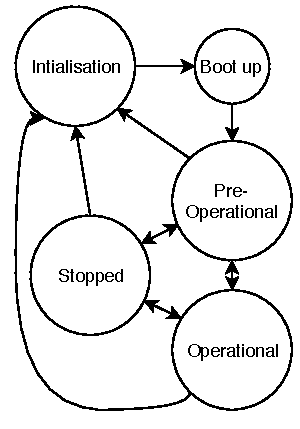
\includegraphics[width=0.3\textwidth]{figures/CANOpen_NMT}
    \vspace{-0.5cm}
    \caption{Device states described in CANOpen specification}
    \label{fig:CANOpen NMT}
    \vspace{-0.5cm}
\end{wrapfigure}
Beside exchange of data CANOpen protocol describes a way to control basic device states. By messages referred as "Network Management" (NMT) one can read device state and send commands to change it. The states and all possible transitions are shown in figure \ref{fig:CANOpen NMT}.

As one can notice to states are restricted to ones important for communication and parameters setting. After the device is on, booting sequence can be started then in a pre-operational state all configuration can be made to finally turn it into operational mode. For instance in connecting to a motor controller, firstly we check communication then turn on pre-charge circuit during boot sequence then setup all necessary parameters (encoder, current limitation etc.) subsequently turning the control loop on.

This is just cover general states but in more complex applications clearly, there are more states to address, however, in this case, there is no argument against using certain objects in the dictionary to control sub-states.

Last but not least, there are 4 more functions cover: Emergency (EMC) - responsible for asynchronous communication of errors, previously mentioned SYNC - to periodically request device state, time stamp - to synchronise devices clock and layer settings services (LSS) - to automatically identify multiple devices on the bus.

All these briefly described functions, collectively provide powerful abstraction over the CAN network standardising way it is used.

\cite{CAN_CIA,CANOpen_NIKHEF,CANOpen_solutions,CANOpen_microcontrol}
\\ \\ \\ \\ \\ \\ 

% \section{Steering - torque vectoring and load sharing}


% \chapter{Existing solutions/ compare to IC vehicles}
% Literature review on recent developments within the topic and techniques used in combustion engine cars